\cleardoublepage
\section{Badanie jakości i wydajności zaproponowanego rozwiązania}

    W ramach pracy przeprowadzono eksperymenty polegające na porównaniu wydajności oraz jakości zaimplementowanych metod do grupowania sekwencji genetycznych w kontekście pełnej klasyfikacji taksonomicznej przeprowadzonej z wykorzystaniem potoku przetwarzania. W eksperymentach jako punkt odniesienia wybrano klasyfikację taksonomiczną wszystkich sekwencji wejściowych bez użycia potoku przetwarzania.

    % ===== ===== ===== =====
    % OPIS ŚRODOWISKA EKSPERYMENTALNEGO
    % ===== ===== ===== =====
    \subsection{Opis środowiska eksperymentalnego}

        Eksperymenty zostały przeprowadzone na maszynie wirtualnej wykorzystującej technologię KVM o specyfikacji podanej poniżej:

        % \subsubsection{Specyfikacja techniczna}\

            \begin{itemize}
                \item {
                    \textbf{System operacyjny:} Ubuntu 22.04 LTS;
                }
                \item {
                    \textbf{Procesor:} 4 rdzenie wirtualne procesora Intel Core i7-6850K;
                }
                \item {
                    \textbf{Pamięć RAM:} 40GB;
                }
                \item {
                    \textbf{Karta graficzna:} Nvidia GeForce GTX 1080 TI;
                }
                \item {
                    \textbf{Dysk:} dysk sieciowy 1 TB z prędkością odczytu 1 Gbps;
                }
                \item {
                    \textbf{Oprogramowanie:} pakiet \texttt{BLAST} w wersji 2.16.0 oraz sterowniki karty graficznej.
                }
            \end{itemize}

    % ===== ===== ===== =====
    % MIARA JAKOŚCI
    % ===== ===== ===== =====
    \subsection{Miara jakości}

        Jako miarę jakości klasyfikacji taksonomicznej wykorzystano zmodyfikowany indeks Jaccarda, wyrażony za pomocą wzoru~\ref{Equation:Quality}.

        \begin{equation}
            \text{Q} = \frac{
                \sum_{r \in (O(R) \cap O(E))} R_{r}
            }{
                \sum_{r \in (O(R) \cup O(E))} R_{r}
            }
            \label{Equation:Quality}
        \end{equation}

        gdzie:
        \begin{align*}
            R &- \text{zbiór wyników referencyjnych,} \\
            E &- \text{zbiór wyników otrzymanych,} \\
            R_{r} &- \text{liczba wyników w zbiorze referencyjnym przypisanych do organizmu $r$,} \\
            O(X) &- \text{zbiór unikalnych organizmów, dla których przypisano wyniki w zbiorze X. }
        \end{align*}

        Miara została wykorzystana do porównania jakości klasyfikacji taksonomicznej przeprowadzanej z wykorzystaniem zaimplementowanych metod względem klasyfikacji taksonomicznej bez użycia potoku przetwarzania.

        Do porównywania jakości wielu przebiegów klasyfikacji taksonomicznej wykorzystano średnią jakość ważoną zdefiniowaną za pomocą wzoru~\ref{Equation:WeightedAverageQuality}.

        \begin{equation}
            Q_{\text{avg}} = \sum_{c \in C} \frac{n_c}{n} Q_c
            \label{Equation:WeightedAverageQuality}
        \end{equation}

        gdzie:
        \begin{align*}
          C &- \text{zbiór wszystkich przebiegów klasyfikacji taksonomicznych,} \\
          Q_c &- \text{jakość klasyfikacji taksonomicznej $c$,} \\
          n_c &- \text{liczba sekwencji wejściowych do klasyfikacji taksonomicznej $c$,}\\
          n   &- \text{liczba sekwencji wejściowych $n = \sum_{c \in C} n_{c}.$}
        \end{align*}

        Wykorzystano również dodatkowe miary jakości, które zostały zastosowane do oceny jakości utworzonych grup przez potok przetwarzania. Pierwszą wykorzystaną miarą jest znormalizowana informacja wzajemna (ang. \textit{Normalized mutual information, NMI}) i służy do oceny jakości grup, drugą jest czułość (ang. \textit{sensitivity}), która wykorzystana jest do oceny reprezentantów grup. Miary zostały zdefiniowane odpowiednio wzorami \eqref{Equation:NMI} i \eqref{Equation:Sensitivity}.

        \begin{equation}
            NMI(X, Y) = \frac{I(X, Y)}{\sqrt{H(X) \cdot H(Y)}}
            \label{Equation:NMI}
        \end{equation}

        gdzie:
        \begin{align*}
            I(X, Y) &= \sum_{y \in Y}{ \sum_{x \in X}{p(x, y) \log_{2}{\frac{p(x, y)}{p(x) p(y)}}}}, \\
            H(X) &= - \sum_{x \in X}{ p(x) \log_{2}{p(x)}}, \\
            I(X, Y) &- \text{informacja wzajemna między zbiorami $X$ oraz $Y$}, \\
            H(X) &- \text{entropia zbioru $X$}, \\
            H(Y) &- \text{entropia zbioru $Y$}, \\
            p(x) &- \text{prawdopodobieństwo zajścia zdarzenia $x$}, \\
            p(x, y) &- \text{wspólny rozkład prawdopodobieństwa $X$ oraz $Y$ }.
        \end{align*}

        \begin{equation}
            sensitivity = \frac{\text{TP}}{
                \text{TP} + \text{TN}
            }
            \label{Equation:Sensitivity}
        \end{equation}

        gdzie:
        \begin{align*}
            TP &- \text{liczba wyników prawdziwie dodatnich,} \\
            TN &- \text{liczba wyników fałszywie ujemnych.}
        \end{align*}

        Dodatkowe miary jakości zostały wykorzystane do oceny jakości względnej między zaimplementowanymi metodami.

    % ===== ===== ===== =====
    % ZBIÓR DANYCH
    % ===== ===== ===== =====
    \subsection{Zbiór danych do badań}

        \subsubsection{Opis zbioru danych}

            W eksperymentach wykorzystano ten sam zbiór sekwencji genetycznych, co w uczeniu modelu sztucznej sieci neuronowej. Zbiór \textit{CAMI II Toy Human Microbiome Project}\cite{Fritz:2019} został wybrany, ponieważ został stworzony w celu oceny wydajności algorytmów bioinformatycznych oraz zawiera znaczną liczbę sekwencji genetycznych, co umożliwiło jego wykorzystanie go zarówno w eksperymentach, jak i w uczeniu modelu sztucznej sieci neuronowej.

            Na podstawie zbioru stworzono podzbiory sekwencji o rozmiarach wyrażonych wzorem $2^k$ dla $k \in [0, 12]$. Zbiory są rozłączne, a do ich budowy wykorzystano wyłącznie te sekwencje, które nie zostały użyte do uczenia modelu sztucznej sieci neuronowej.

        \subsubsection{Przygotowanie zbioru danych}

            Podzbiory powstały poprzez losowanie bez zwracania indeksów sekwencji genetycznych ze zbioru referencyjnego, które powinny trafić do podzbioru. W losowaniu wykorzystano informację o indeksach sekwencji wykorzystanych w zbiorze uczącym oraz walidacyjnym sztucznej sieci neuronowej. W celu umożliwienia dalszego wykorzystania zbioru danych zapisano do pliku indeksy sekwencji wykorzystanych w procesie budowy zbioru eksperymentalnego. Podzbiory sekwencji zostały zapisane do plików w formacie FASTA.

    % ===== ===== ===== =====
    % PROCEDURA PRZEPROWADZANIA EKSPERYMENTÓW
    % ===== ===== ===== =====
    \subsection{Procedura przeprowadzania eksperymentów}

        Eksperymenty zostały przeprowadzone za pomocą zaimplementowane polecenia aplikacji konsolowej \texttt{experiment}, które pozwala na nadzorowanie wykorzystania procesora oraz pamięci RAM przez polecenie, oraz kontrolowanie maksymalnego czasu trwania wykonywanego polecenia.

        Dane do obu eksperymentów zostały zgromadzone w wyniku przeprowadzenia klasyfikacji taksonomicznej z wykorzystaniem zaimplementowanych metod oraz klasyfikacji taksonomicznej bez wykorzystania potoku przetwarzania dla każdego podzbioru osobno.

        W wyniku przeprowadzonych klasyfikacji taksonomicznych otrzymano informację o przebiegu procesu w formie plików z rozszerzeniem \texttt{.experiment}, zawierających dane dotyczące wykorzystania zasobów podczas przebiegu klasyfikacji oraz czasu jej trwania. W przypadku sukcesu procesu grupowania otrzymano plik z rozszerzeniem \texttt{.clusters}, który zawiera informację o stworzonych grupach. Natomiast w przypadku pomyślnej klasyfikacji taksonomicznej końcowe wyniki całego procesu zapisano do pliku z rozszerzeniem \texttt{.search}.

        \subsubsection{Parametry}

            Maksymalny czas trwania jednej klasyfikacji taksonomicznej został ograniczony do 12 godzin. Dla wszystkich metod wybrano algorytm grupowania $k$-medoidów oraz określono liczbę tworzonych grup przez algorytm grupowania za pomocą wzoru $\sqrt{n}$, gdzie $n$ to liczba sekwencji wejściowych. W metodzie z wykorzystaniem zmodyfikowanego algorytmu Needlemana-Wunscha wykorzystano parametry określone w sekcji~\ref{Method:NeedlemanWunsch}. W przypadku metody wykorzystującej zanurzenia $k$-merów parametr $k$ został ustawiony na $4$. W metodzie z wykorzystaniem sztucznej sieci neuronowej wykorzystano wcześniej stworzony model.

        \subsubsection{Skrypty}

            Do przeprowadzenia eksperymentów zostały wykorzystane opracowane skrypty w języku \texttt{bash}. Każdy skrypt uruchamia klasyfikację taksonomiczną dla podzbiorów z wykorzystaniem jednej metody.

            \begin{itemize}
                \item {
                    Skrypt \texttt{experiment\_default\_search.sh} uruchamia klasyfikacją taksonomiczną bez wykorzystania potoku przetwarzania.
                }
                \item {
                    Skrypt \texttt{experiment\_needleman\_wunsch.sh} uruchamia klasyfikacją taksonomiczną z wykorzystaniem zmodyfikowanego algorytmu Needlemana-Wunscha.
                }
                \item {
                    Skrypt \texttt{experiment\_kmer.sh} uruchamia klasyfikacją taksonomiczną z wykorzystaniem zanurzeń $k$-merów.
                }
                \item {
                    Skrypt \texttt{experiment\_neural.sh} uruchamia klasyfikacją taksonomiczną z wykorzystaniem modelu sztucznej sieci neuronowej.
                }
            \end{itemize}

            Uruchomienie wszystkich skryptów pozwala na zebranie wszystkich danych dla obu eksperymentów. Do przetworzenia wyników z uruchomienia skryptów oraz wygenerowania wykresów wykorzystano skrypt stworzony w języku \texttt{Python}. Skrypt \texttt{plot\_experiments.py} pozwala na wygenerowanie i zapisanie wykresów dla obu eksperymentów.

    % ===== ===== ===== =====
    % WYNIKI
    % ===== ===== ===== =====
    \subsection{Wyniki i wnioski}

        \subsubsection{Eksperyment 1: Czas wykonania klasyfikacji taksonomicznej}

            \paragraph{Cel}
                Celem eksperymentu jest sprawdzanie czasu wykonania klasyfikacji taksonomicznej przy użyciu różnych metod grupowaniu sekwencji genetycznych.

            \paragraph{Założenia}
                \begin{enumerate}
                    \item {
                        Proces tworzenia grup przebiega deterministycznie.
                    }
                    \item {
                        Klasyfikacja taksonomiczna jest jedynym zadaniem wykonywanym na maszynie eksperymentalnej.
                    }
                    \item {
                        Rozdzielczość monitorowania ustawiono na 5 sekund, co skutkuje dokładnością raportowanych czasów na $\pm 5$ sekund.
                    }
                \end{enumerate}

            \paragraph{Wyniki}
                W wyniku przeprowadzonych eksperymentów otrzymano czas wykonania klasyfikacji taksonomicznej dla wszystkich metod. W przypadku metody wykorzystującej zmodyfikowany algorytm Needlemana-Wunscha nie udało się otrzymać wyników dla klasyfikacji taksonomicznej $4096$ sekwencji z powodu przekroczenia czasu wykonania. Na rysunku~\ref{Picture:Experiment:Duration} przedstawiono wykres czasu wykonania klasyfikacji taksonomicznej w zależności od ilości sekwencji wejściowych dla: metody ze zmodyfikowanym algorytmem Needlemana-Wunscha (NW), metody wykorzystującej zanurzenia $k$-merów ($k$-mer), metody wykorzystującej sztuczne sieci neuronowe (SSN) oraz dla klasyfikacji taksonomicznej wszystkich sekwencji bez wykorzystania potoku (BZ). Szczegółowe czasy wykonania zostały zawarte w tabeli~\ref{Table:Experiment:Duration}. Ze względu na monitorowanie wykorzystania procesora oraz pamięci RAM przez klasyfikację, zgromadzono także dane o średnim wykorzystaniu procesora oraz maksymalnej użytej pamięci. Wyniki te zostały przedstawione w tabeli~\ref{Table:Experiment:Resources}.

                \begin{figure}[!htb]
                    \begin{center}
                        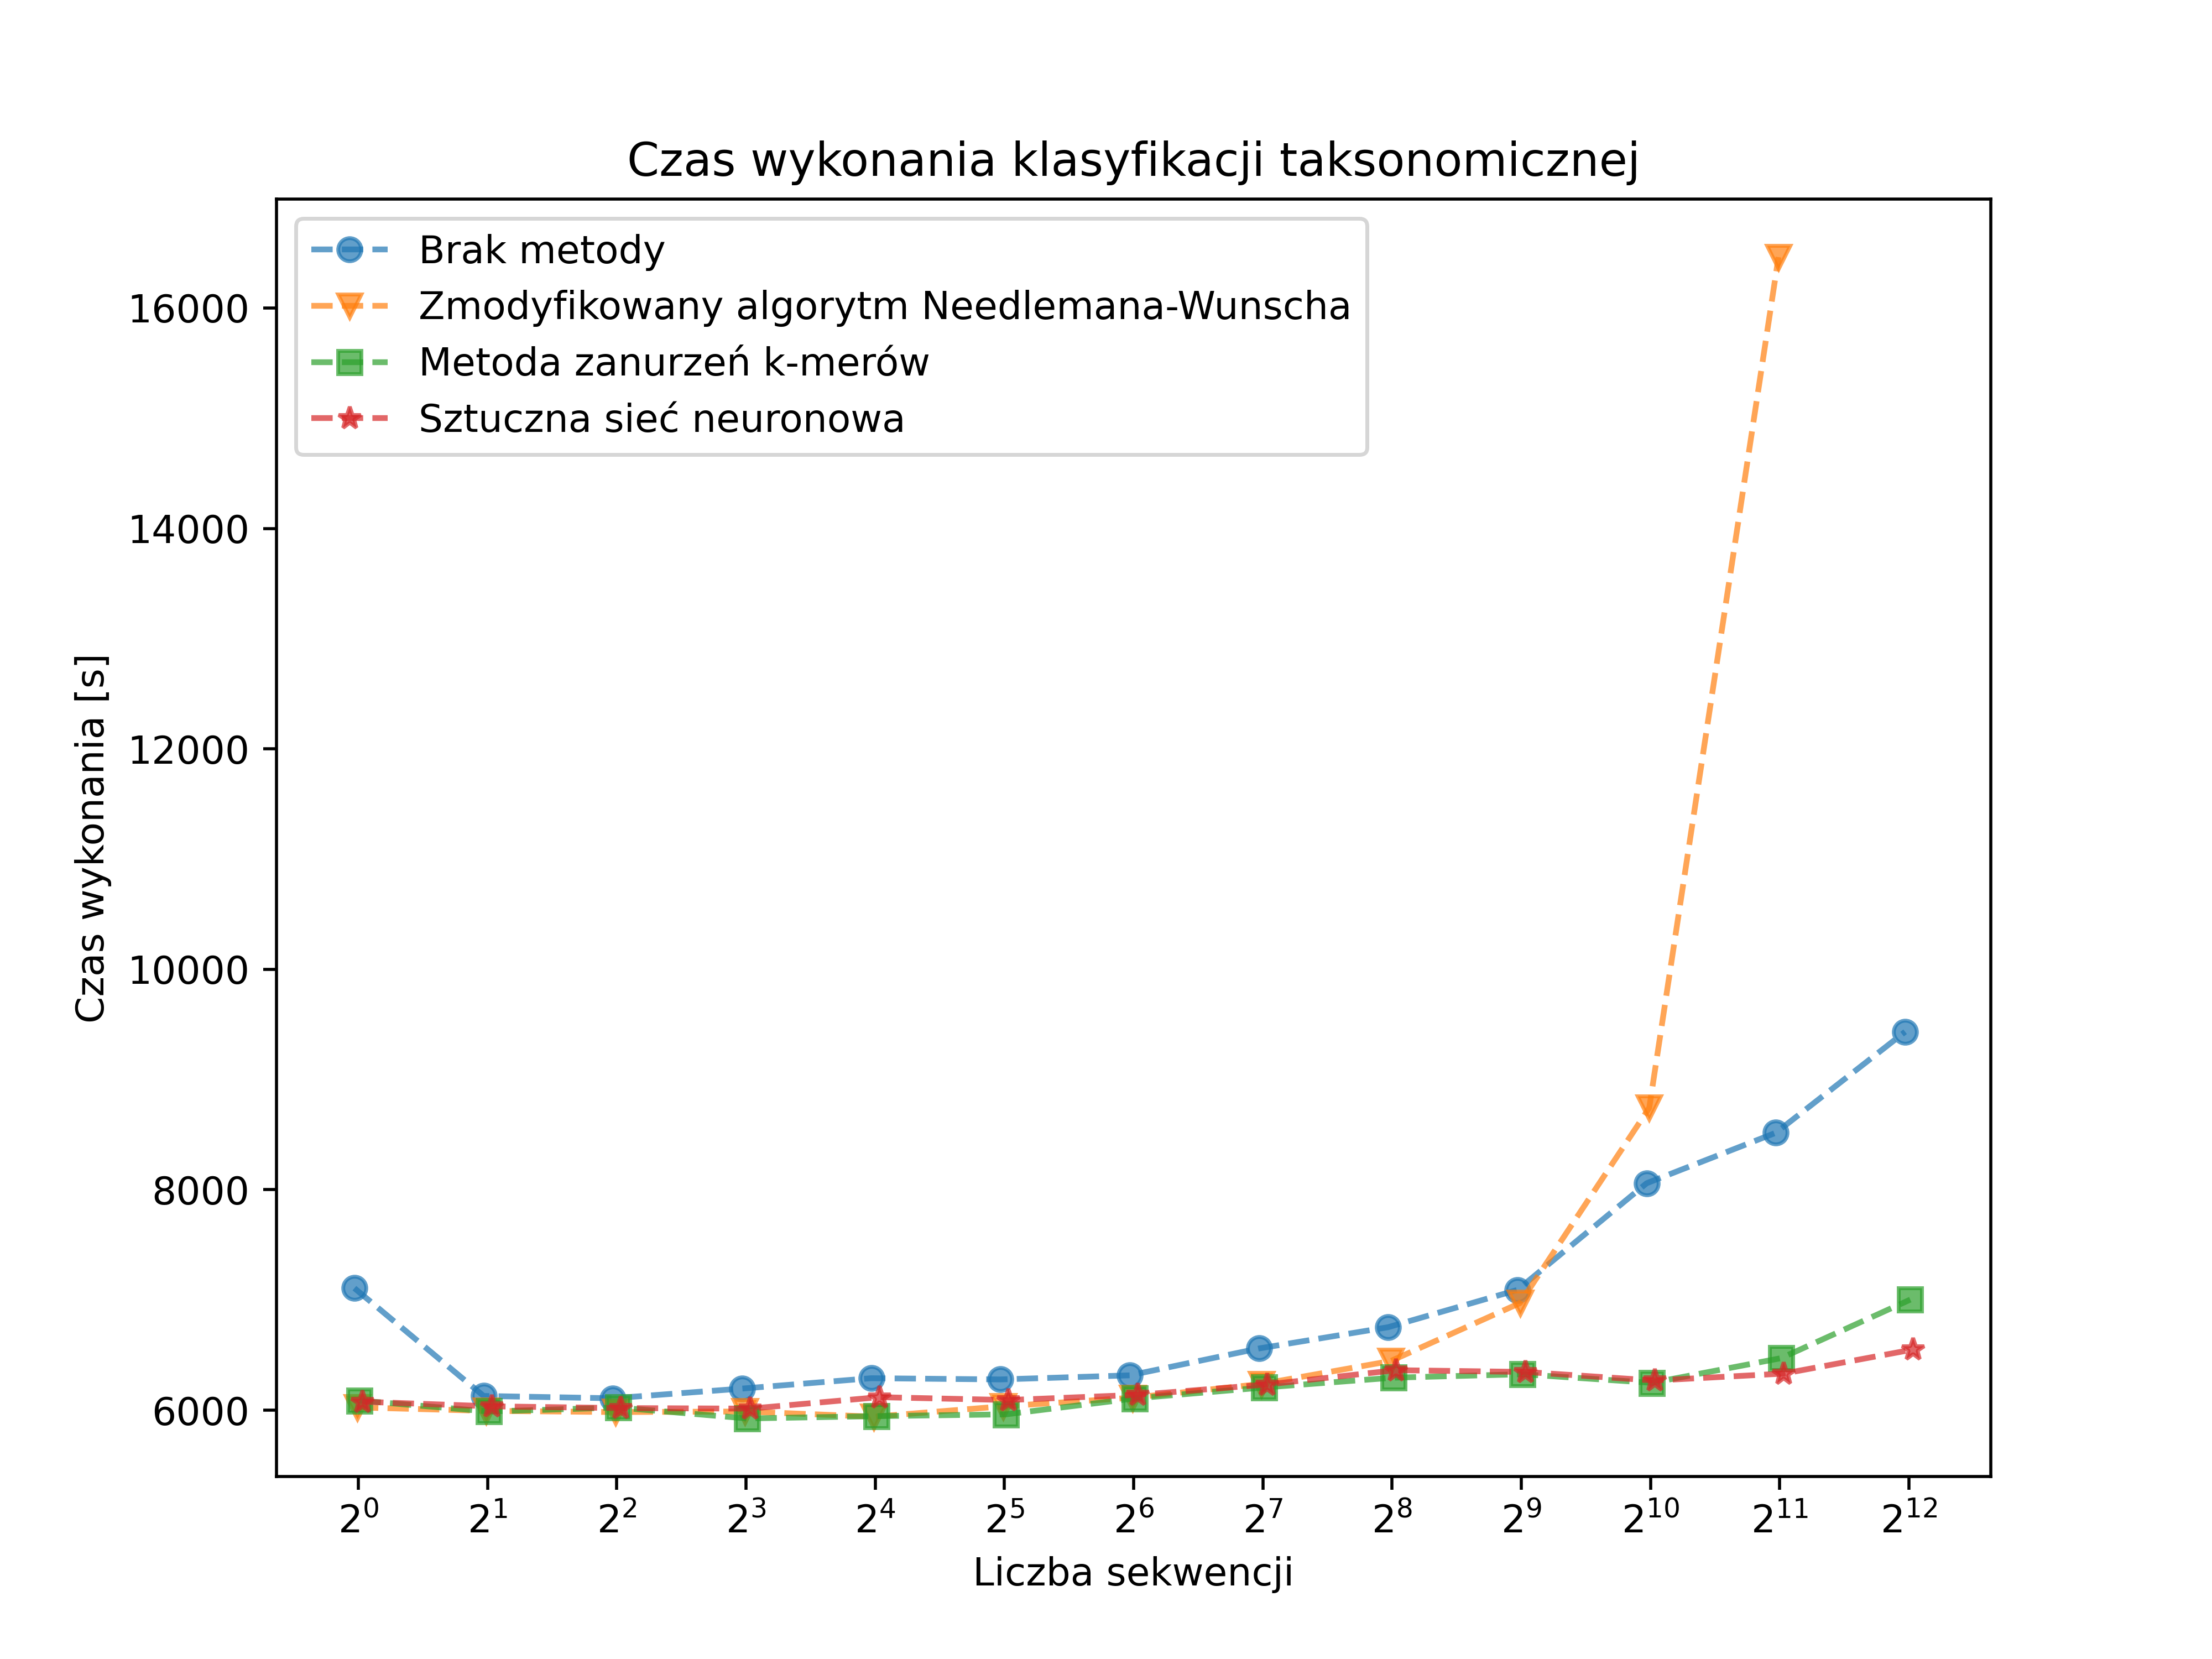
\includegraphics[width=\textwidth]{tex/pictures/exp/experiment_duration.png}
                    \end{center}
                    \caption{
                        Czas wykonania klasyfikacji taksonomicznej.
                    }\label{Picture:Experiment:Duration}
                \end{figure}

                \begin{table}\centering
                    \caption{Czas trwania eksperymentów.}\label{Table:Experiment:Duration}
                    \begin{tabularx}{\textwidth}{|c||R|R|R|R|}
                        \hline
                        \multirow{2}{*}{\textbf{Liczba sekwencji}} & \multicolumn{4}{|c|}{\textbf{Czas trwania eksperymentu}} \\ \cline{2-5}
                                        & \textbf{BZ} & \textbf{NW} & \textbf{$k$-mer} & \textbf{SSN} \\ \hline \hline
                                        1 & 7107 & \textbf{6025} & 6087 & 6077\\ \hline
                                        2 & 6129 & 5994 & \textbf{5988} & 6035\\ \hline
                                        4 & 6108 & \textbf{5983} & 6024 & 6019\\ \hline
                                        8 & 6196 & 5988 & \textbf{5925} & 6014\\ \hline
                                        16 & 6290 & \textbf{5941} & 5946 & 6118\\ \hline
                                        32 & 6279 & 6035 & \textbf{5962} & 6092\\ \hline
                                        64 & 6316 & 6113 & \textbf{6107} & 6139\\ \hline
                                        128 & 6560 & 6238 & \textbf{6206} & 6233\\ \hline
                                        256 & 6753 & 6446 & \textbf{6295} & 6363\\ \hline
                                        512 & 7091 & 6972 & \textbf{6326} & 6347\\ \hline
                                        1024 & 8059 & 8743 & \textbf{6248} & 6269\\ \hline
                                        2048 & 8517 & 16461 & 6472 & \textbf{6332}\\ \hline
                                        4096 & 9433 & \textbf{-1} & 7003 & 6550\\ \hline

                    \end{tabularx}
                \end{table}

                \begin{table}\centering
                    \caption{Wykorzystanie procesora oraz pamięci.}\label{Table:Experiment:Resources}
                    \begin{tabularx}{\textwidth}{|c||R|R|R|R||R|R|R|R|}
                        \hline
                        \multirow{2}{*}{\textbf{Liczba sekwencji}} & \multicolumn{4}{|c||}{\textbf{Wykorzystanie procesora [proc.]}} & \multicolumn{4}{|c|}{\textbf{Wykorzystanie pamięci [MB]}} \\ \cline{2-9}
                                        & \textbf{BZ} & \textbf{NW} & \textbf{$k$-mer} & \textbf{SSN} & \textbf{BZ} & \textbf{NW} & \textbf{$k$-mer} & \textbf{SSN} \\ \hline \hline
                                        1 & \textbf{14} & \textbf{14} & \textbf{14} & \textbf{14} & 37954 & 37451 & 39191 & \textbf{41120}\\ \hline
                                        2 & \textbf{15} & 14 & 14 & 14 & 37584 & 37493 & 38081 & \textbf{40567}\\ \hline
                                        4 & \textbf{16} & 14 & 14 & 14 & 37632 & 37510 & 38150 & \textbf{40701}\\ \hline
                                        8 & \textbf{18} & 14 & 15 & 13 & 37590 & 37545 & 38119 & \textbf{40685}\\ \hline
                                        16 & \textbf{22} & 15 & 16 & 17 & 37596 & 37509 & 38133 & \textbf{40781}\\ \hline
                                        32 & \textbf{21} & 15 & 16 & 15 & 37846 & 37589 & 38115 & \textbf{40766}\\ \hline
                                        64 & \textbf{21} & 17 & 17 & 17 & 37798 & 37604 & 37963 & \textbf{40706}\\ \hline
                                        128 & \textbf{26} & 21 & 20 & 19 & 37476 & 37638 & 37973 & \textbf{40396}\\ \hline
                                        256 & \textbf{32} & 25 & 22 & 20 & 37539 & 37667 & 37957 & \textbf{40385}\\ \hline
                                        512 & \textbf{38} & 33 & 25 & 23 & 37465 & 37590 & 37929 & \textbf{40414}\\ \hline
                                        1024 & \textbf{53} & 44 & 21 & 19 & 37462 & 37591 & 37876 & \textbf{40490}\\ \hline
                                        2048 & 61 & \textbf{70} & 24 & 22 & 37424 & 37607 & \textbf{37907} & 33674\\ \hline
                                        4096 & 68 & \textbf{96} & 29 & 24 & 37463 & 37504 & \textbf{37900} & 17106\\ \hline
                    \end{tabularx}
                \end{table}

            \paragraph{Wnioski}
                Metoda z wykorzystaniem zmodyfikowanego algorytmu Needlemana-Wunscha zgodnie z oczekiwaniami cechowała się najszybszym wzrostem czasu wykonania klasyfikacji taksonomicznej. Gwałtowny wzrost spowodowany jest porównywanie sekwencji każda z każdą przez budowę macierzy podobieństwa. Pomimo redukcji ilości sekwencji, które poddawane są klasyfikacji, czas wykonania tą metodą przekroczył klasyfikację taksonomiczną wszystkich sekwencji bez wykorzystania potoku przetwarzania.

                Metody z wykorzystaniem zanurzeń $k$-merów oraz sztucznej sieci neuronowej cechowały się porównywalnymi czasami wykonania z lekką przewagą dla pierwszej metody. Obie metody działały szybciej od klasyfikacji taksonomicznej bez wykorzystania potoku przetwarzania. Metody do porównywania wykorzystują reprezentacje sekwencji, co spowodowało powolniejszy wzrost czasu wykonania klasyfikacji taksonomicznej. W przypadku metody ze sztuczną siecią neuronową krótszy czas wykonania dla $4096$ sekwencji może być spowodowany obliczaniem zanurzeń dla wszystkich sekwencji jednocześnie za pomocą karty graficznej.

                W przypadku wykorzystania zasobów zauważono wzrost średniego wykorzystania procesora przez klasyfikację taksonomiczną z wykorzystaniem zaimplementowanych metod w miarę wzrostu czasu wykonania klasyfikacji, co jest związane ze znacznym nakładem obliczeniowym podczas tworzenia macierzy niepodobieństwa, której złożoność tworzenia rośnie kwadratowo wraz z liczbą sekwencji.

                Zauważalne również jest większe wykorzystanie pamięci RAM przez metodę ze sztuczną siecią neuronową, co spowodowane jest koniecznością wczytania modelu sztucznej sieci neuronowej do pamięci.

        \subsubsection{Eksperyment 2: Jakość klasyfikacji taksonomicznej}

            \paragraph{Cel}
                Celem drugiego eksperymentu było zbadanie jakości klasyfikacji taksonomicznej z wykorzystaniem zaimplementowanych metod względem klasyfikacji taksonomicznej wszystkich sekwencji. Zbadano również tworzone grupy przez zaimplementowane metody.

            \paragraph{Założenia}

                \begin{enumerate}
                    \item {
                        Proces tworzenia grup przebiega deterministycznie.
                    }
                    \item {
                        Program \texttt{BLASTn} działa deterministycznie, zwracając dla danej sekwencji i zadanych parametrów zawsze te same wyniki.
                    }
                    \item {
                        W przypadku braku możliwości obliczenia jakości dla danego przebiegu klasyfikacji taksonomicznej za wartość jakości przyjęto $0$, wartość ta nie jest brana pod uwagę w przypadku obliczania średniej jakości ważonej.
                    }
                \end{enumerate}

            \paragraph{Wyniki}
                Obliczono jakość klasyfikacji za pomocą miary wyrażonej wzorem~\ref{Equation:Quality} dla zaimplementowanych metod względem pełnej klasyfikacji taksonomicznej. Na rysunku~\ref{Picture:Experiment:Quality} przedstawiono wykres jakości klasyfikacji w zależności od ilości sekwencji wejściowych, szczegółowe wyniki jakości umieszczono w tabeli~\ref{Table:Experiment:Quality}. Średnia ważona jakość obliczona za pomocą wzoru~\ref{Equation:WeightedAverageQuality} dla metody ze zmodyfikowanym algorytmem Needlemana-Wunscha wyniosła $0,899$, dla metody z zanurzeniami $k$-merów wyniosła $0,921$, natomiast dla metody z wykorzystaniem sztucznej sieci neuronowej $0,944$. Na rysunku~\ref{Picture:Experiment:RelativeQualityNMI} przedstawiono wykres jakości względnej grup obliczony za pomocą wzoru~\ref{Equation:NMI}, natomiast na rysunku~\ref{Picture:Experiment:RelativeQualitySensitivity} przedstawiono wykres czułości obliczonej za pomocą wzoru~\ref{Equation:Sensitivity} reprezentantów grup. Szczegółowe wyniki znajdują się odpowiednio w tabeli~\ref{Table:Experiment:RelativeQualityNMI} oraz tabeli~\ref{Table:Experiment:RelativeQualitySensitivity}.

                \begin{figure}[!htb]
                    \begin{center}
                        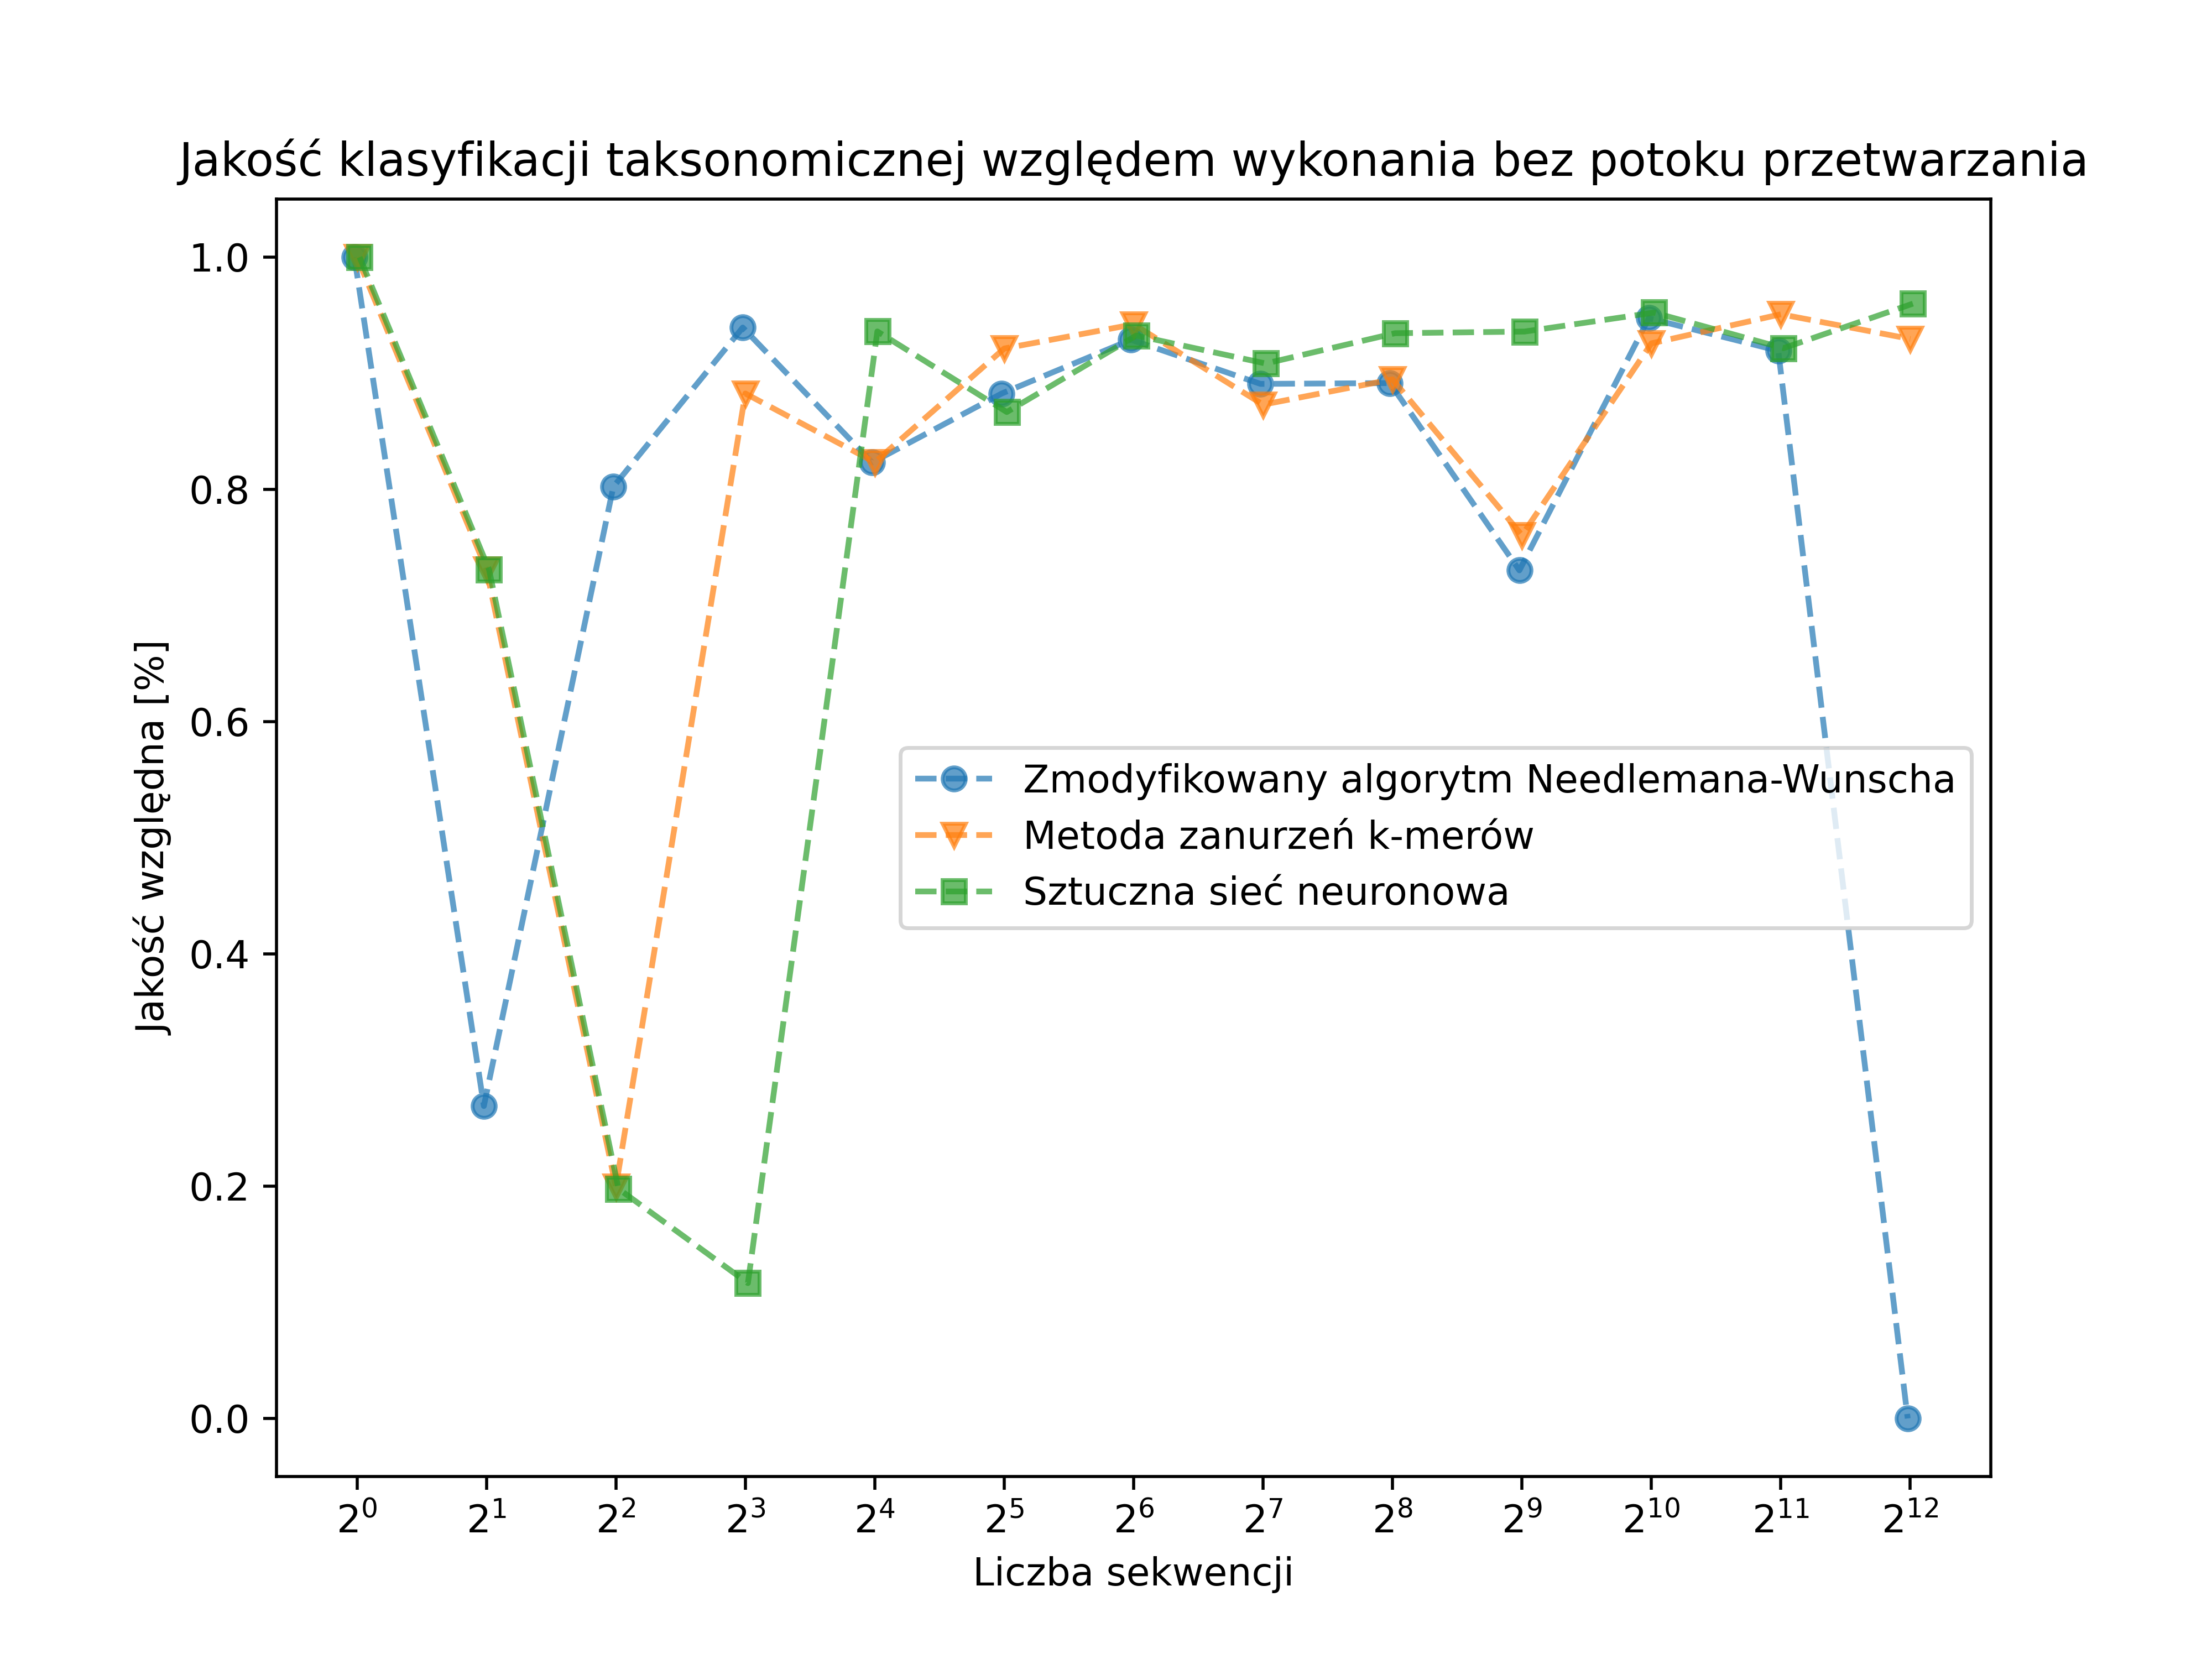
\includegraphics[width=\textwidth]{tex/pictures/exp/experiment_quality.png}
                    \end{center}
                    \caption{
                        Jakość klasyfikacji taksonomicznej.
                    }\label{Picture:Experiment:Quality}
                \end{figure}

                \begin{table}\centering
                    \caption{Jakość klasyfikacji taksonomicznej.}\label{Table:Experiment:Quality}

                    \begin{tabularx}{\textwidth}{|c|R|R|R|}
                        \hline
                        \multirow{2}{*}{\textbf{Liczba sekwencji}} & \multicolumn{3}{|c|}{\textbf{Metoda}} \\ \cline{2-4}
                        & \textbf{NW} & \textbf{$k$-mer} & \textbf{SSN} \\ \hline \hline
                        1 & \textbf{1,0} & \textbf{1,0} & \textbf{1,0}\\ \hline
                        2 & 0,27 & \textbf{0,73} & \textbf{0,73}\\ \hline
                        4 & \textbf{0,8} & 0,2 & 0,2\\ \hline
                        8 & \textbf{0,94} & 0,88 & 0,12\\ \hline
                        16 & 0,82 & 0,82 & \textbf{0,94}\\ \hline
                        32 & 0,88 & \textbf{0,92} & 0,87\\ \hline
                        64 & 0,93 & \textbf{0,94} & 0,93\\ \hline
                        128 & 0,89 & 0,87 & \textbf{0,91}\\ \hline
                        256 & 0,89 & 0,89 & \textbf{0,93}\\ \hline
                        512 & 0,73 & 0,76 & \textbf{0,94}\\ \hline
                        1024 & \textbf{0,95} & 0,93 & \textbf{0,95}\\ \hline
                        2048 & 0,92 & \textbf{0,95} & 0,92\\ \hline
                        4096 & 0,0 & 0,93 & \textbf{0,96}\\ \hline
                    \end{tabularx}
                \end{table}

                \begin{figure}[!htb]
                    \begin{center}
                        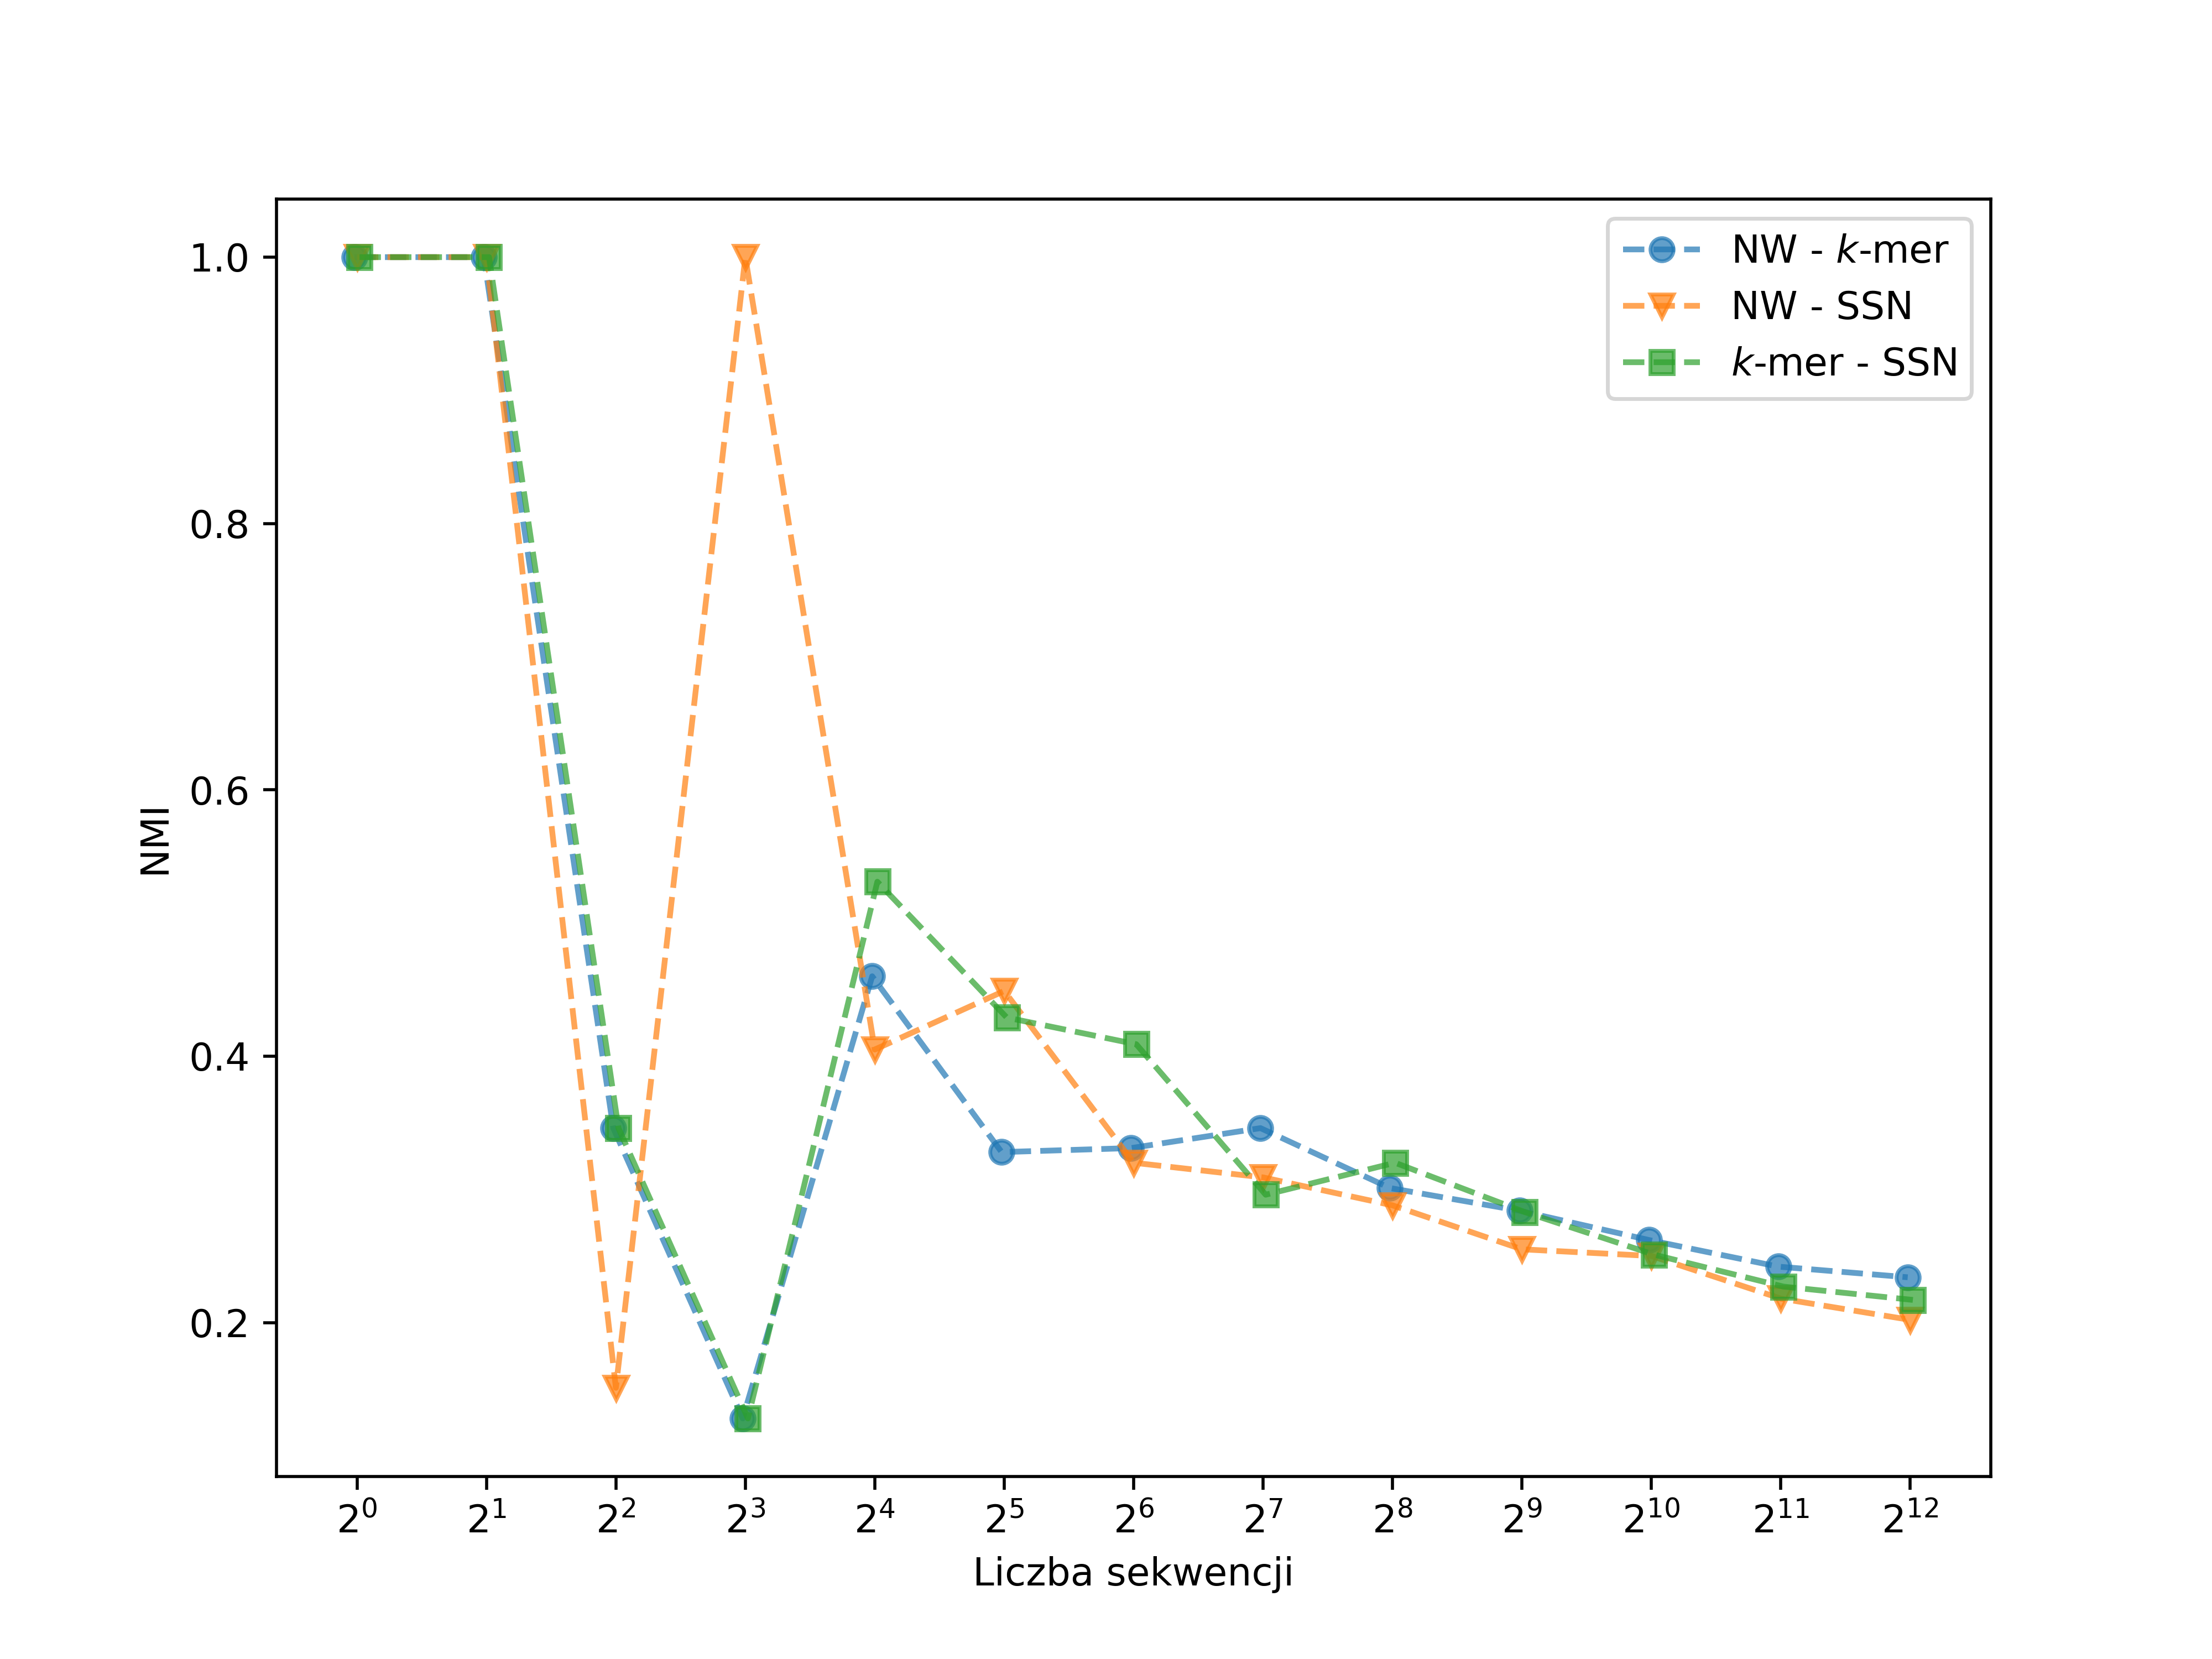
\includegraphics[width=\textwidth]{tex/pictures/exp/experiment_relative_quality_nmi.png}
                    \end{center}
                    \caption{
                       Jakość względna grup wykorzystywanych w klasyfikacji taksonomicznej.
                    }\label{Picture:Experiment:RelativeQualityNMI}
                \end{figure}

                \begin{figure}[!htb]
                    \begin{center}
                        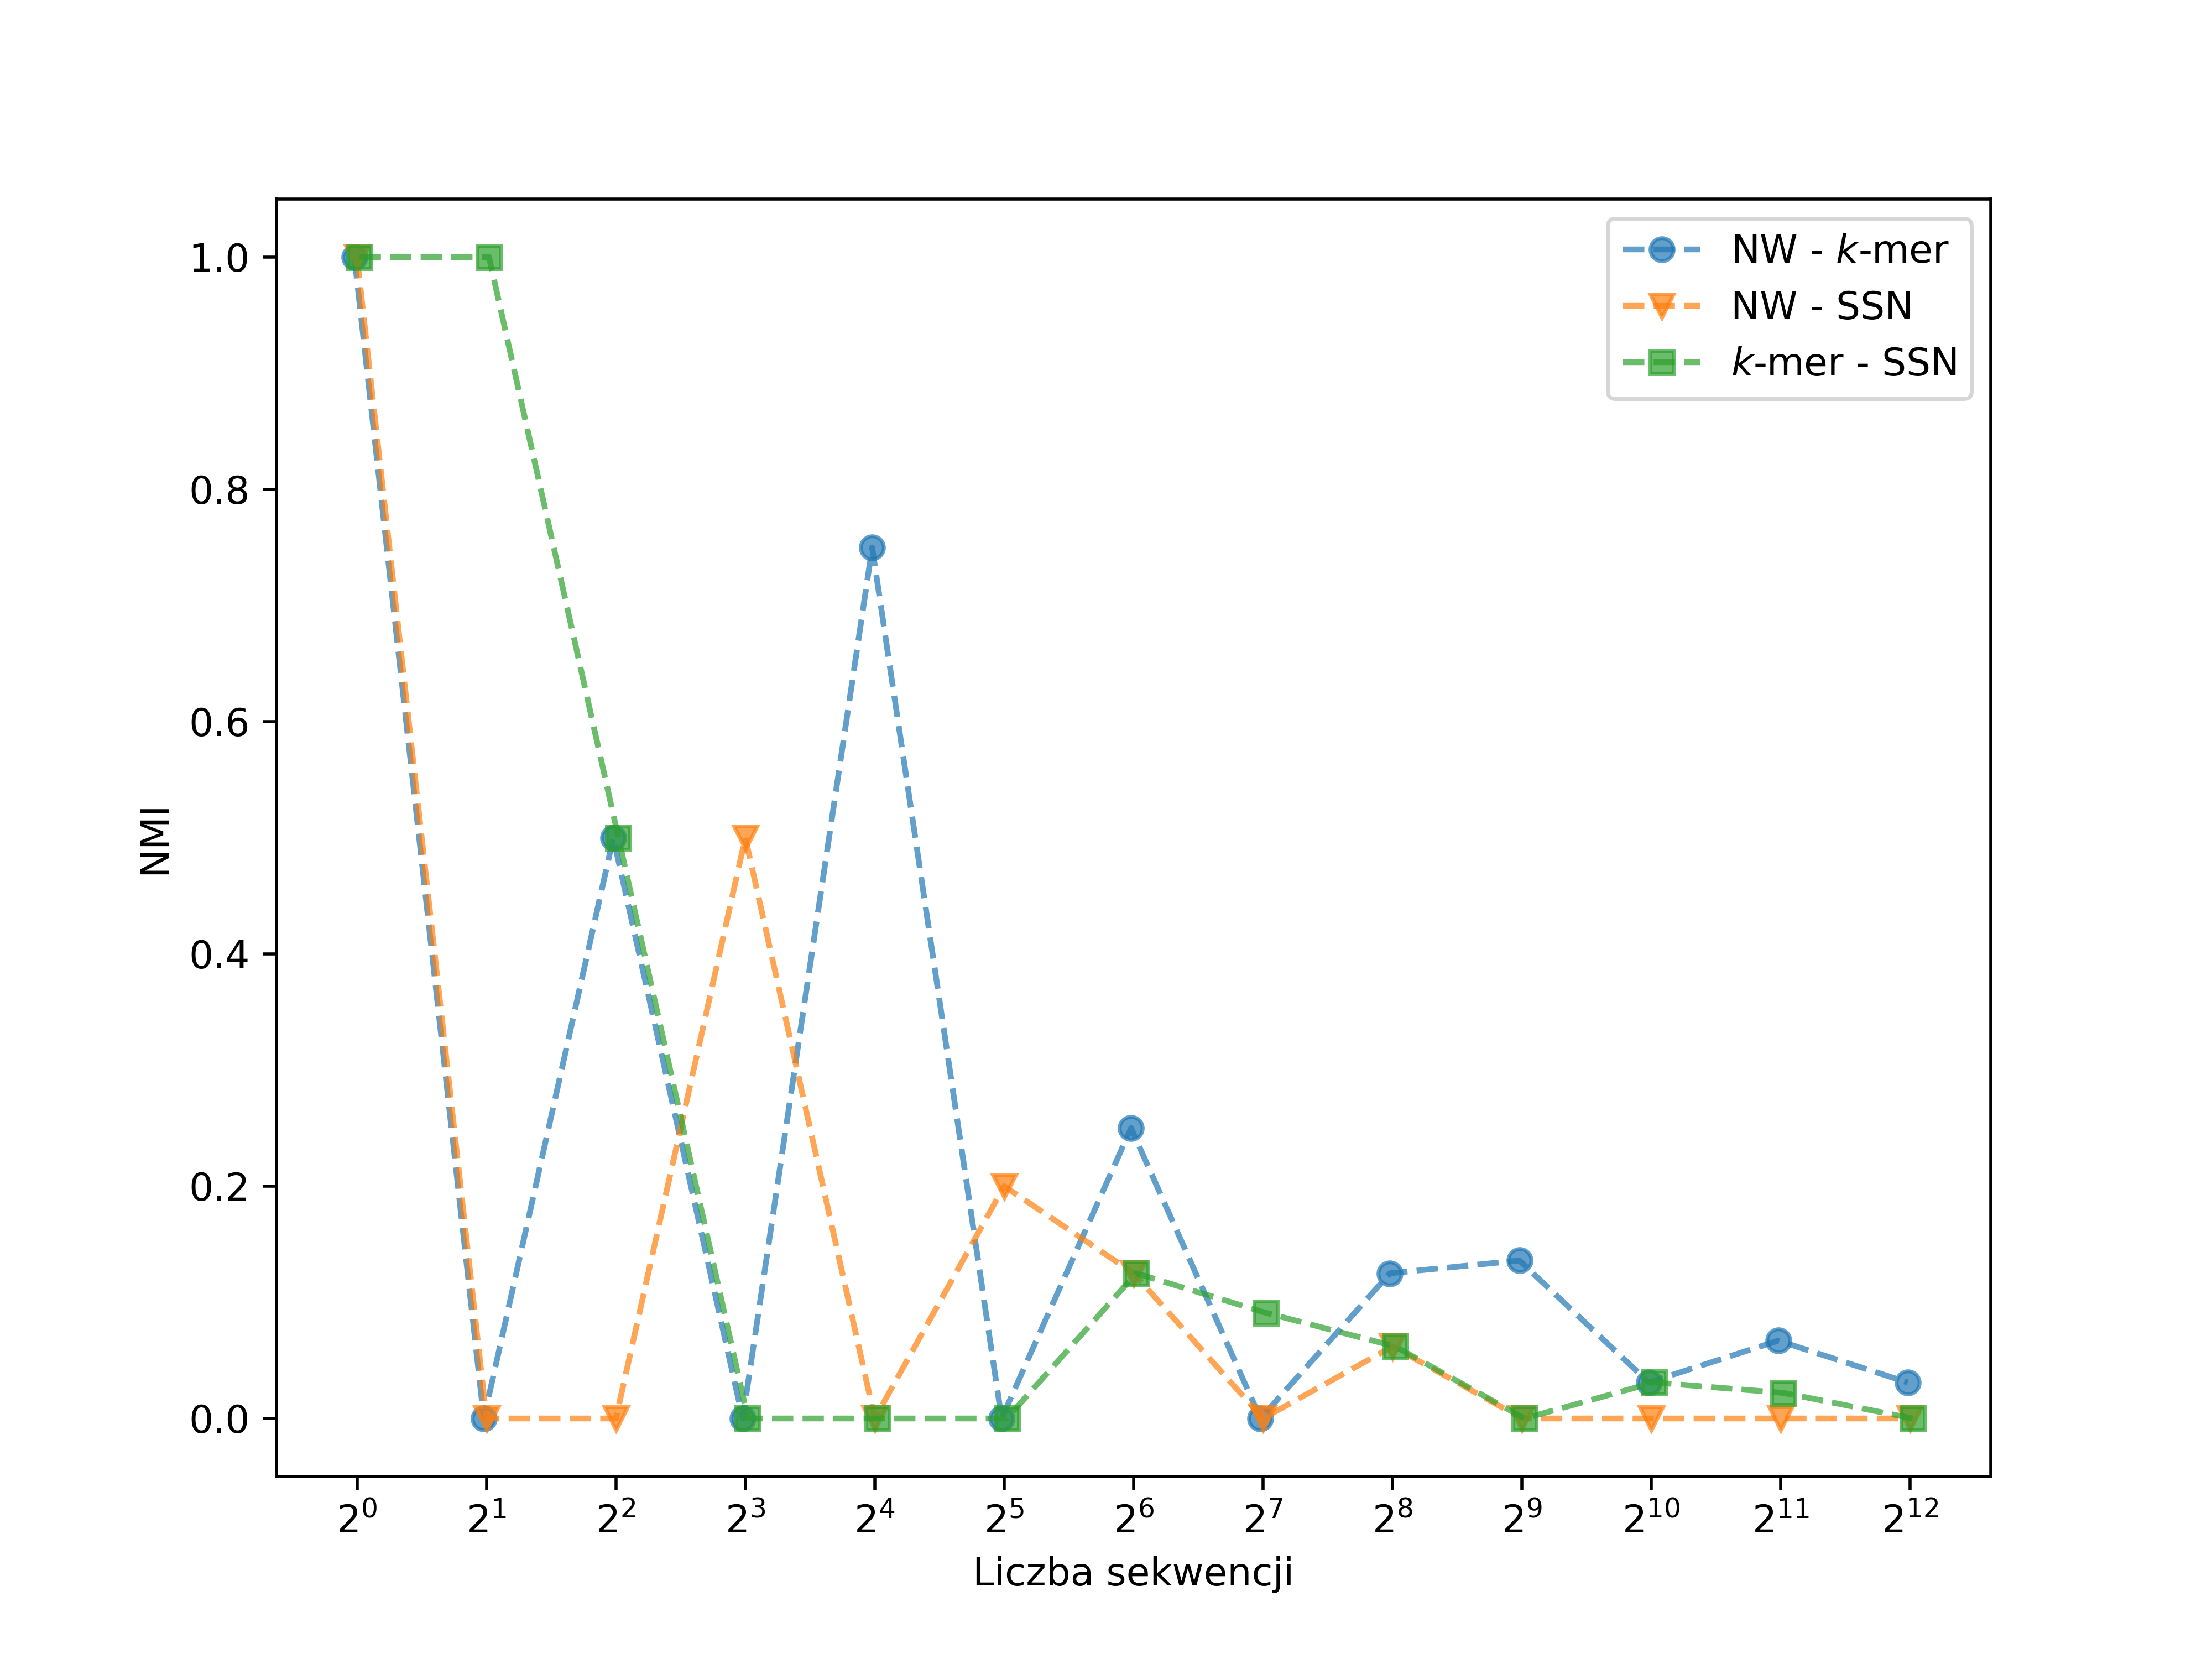
\includegraphics[width=\textwidth]{tex/pictures/exp/experiment_relative_quality_sensitivity.png}
                    \end{center}
                    \caption{
                       Czułość między reprezentantami grup wykorzystanych w klasyfikacji taksonomicznej.
                    }\label{Picture:Experiment:RelativeQualitySensitivity}
                \end{figure}

                \begin{table}\centering
                    \caption{Jakość względna grup wykorzystywanych w klasyfikacji taksonomicznej.}\label{Table:Experiment:RelativeQualityNMI}

                    \begin{tabularx}{\textwidth}{|c|R|R||R|}
                        \hline
                        \multirow{2}{*}{\textbf{Liczba sekwencji}} & \multicolumn{3}{|c|}{\textbf{Metoda}} \\ \cline{2-4}
                        & \textbf{NW - $k$-mer} & \textbf{NW - SSN} & \textbf{$k$-mer - SSN} \\ \hline \hline
                        1 & 1 & 1 & 1\\ \hline
                        2 & 1 & 1 & 1\\ \hline
                        4 & 0,346 & 0,151 & 0,346\\ \hline
                        8 & 0,128 & 1,0 & 0,128\\ \hline
                        16 & 0,46 & 0,405 & 0,531\\ \hline
                        32 & 0,328 & 0,449 & 0,429\\ \hline
                        64 & 0,331 & 0,32 & 0,409\\ \hline
                        128 & 0,346 & 0,309 & 0,296\\ \hline
                        256 & 0,301 & 0,288 & 0,32\\ \hline
                        512 & 0,284 & 0,255 & 0,283\\ \hline
                        1024 & 0,262 & 0,25 & 0,251\\ \hline
                        2048 & 0,242 & 0,218 & 0,227\\ \hline
                        4096 & 0,234 & 0,202 & 0,217\\ \hline
                    \end{tabularx}
                \end{table}

                \begin{table}\centering
                    \caption{Czułość między reprezentantami grup wykorzystanych w klasyfikacji taksonomicznej.}\label{Table:Experiment:RelativeQualitySensitivity}

                    \begin{tabularx}{\textwidth}{|c|R|R||R|}
                        \hline
                        \multirow{2}{*}{\textbf{Liczba sekwencji}} & \multicolumn{3}{|c|}{\textbf{Metoda}} \\ \cline{2-4}
                        & \textbf{NW - $k$-mer} & \textbf{NW - SSN} & \textbf{$k$-mer - SSN} \\ \hline \hline
                        1 & 1,0 & 1,0 & 1,0\\ \hline
                        2 & 0,0 & 0,0 & 1,0\\ \hline
                        4 & 0,5 & 0,0 & 0,5\\ \hline
                        8 & 0,0 & 0,5 & 0,0\\ \hline
                        16 & 0,75 & 0,0 & 0,0\\ \hline
                        32 & 0,0 & 0,2 & 0,0\\ \hline
                        64 & 0,25 & 0,125 & 0,125\\ \hline
                        128 & 0,0 & 0,0 & 0,091\\ \hline
                        256 & 0,125 & 0,062 & 0,062\\ \hline
                        512 & 0,136 & 0,0 & 0,0\\ \hline
                        1024 & 0,031 & 0,0 & 0,031\\ \hline
                        2048 & 0,067 & 0,0 & 0,022\\ \hline
                        4096 & 0,031 & 0,0 & 0,0\\ \hline
                    \end{tabularx}
                \end{table}

            \paragraph{Wnioski}
                Wszystkie zaimplementowane metody osiągnęły bardzo dobre wyniki jakości klasyfikacji, przekraczając $0,7$, w przypadkach, gdy liczba grup była znacznie większa od ilości sekwencji wejściowych. Średnia jakość ważona dla wszystkich metod również osiągnęła wysoką wartość.
                Metoda z wykorzystaniem sztucznej sieci neuronowej osiągnęła najlepszy wynik średniej jakości ważonej, wyprzedzając nieznacznie metodę z zanurzeniami $k$-merów oraz metodę ze zmodyfikowanym algorytmem Needlamana-Wunscha. Wbrew oczekiwaniom, metoda Needlemana-Wunscha osiągnęła najniższy wynik spośród zaimplementowanych metod.
                Metoda z wykorzystaniem sztucznej sieci neuronowej zawdzięcza swój wynik uwzględnieniu pełnej struktury sekwencji przez model, co pozwoliło na lepsze określenie niepodobieństwa między sekwencjami.
                Powolny spadek znormalizowanej informacji wzajemnej wraz ze wzrostem ilości sekwencji wejściowych świadczy o tworzeniu coraz mniej podobnych grup przez algorytm grupowania w wyniku zastosowania różnych metod do wyznaczania niepodobieństwa. Najbardziej podobne zbiory grup były tworzone między metodą ze zmodyfikowanym algorytmem Needlemana-Wunscha a metodą z zanurzeniami $k$-merów.

        \subsubsection{Analiza wyników}

            Wyniki eksperymentów częściowo potwierdziły oczekiwania postawione na początku badań. Wszystkie metody osiągnęły zadowalającą jakość klasyfikacji taksonomicznej. Szczególnie dobrze wypadła metoda wykorzystująca sztuczną sieć neuronową, która osiągnęła najlepszą średnią ważoną jakość klasyfikacji jednocześnie zachowując czas wykonania porównywalny z metodą opartą na zanurzeniach $k$-merów. Metoda Needlemana-Wunscha nie spełniła oczekiwań, będąc najwolniejszą metodą i osiągając wbrew oczekiwaniom jednocześnie najgorsze wyniki jakości klasyfikacji. Niska jakość klasyfikacji taksonomicznej przy małej liczbie sekwencji wejściowych może wynikać z nieodpowiedniego wyboru reprezentantów grup, co jest spowodowane zbyt małą liczbą dostępnych sekwencji. Zaimplementowane metody powinny być więc stosowane jedynie w przypadkach, gdy liczba sekwencji wejściowych przekracza pewien próg i ich wykorzystanie realnie skraca czas procesu klasyfikacji taksonomicznej. Dla badanych danych warunek ten jest osiągnięty dla $128$ sekwencji, gdzie jakość klasyfikacji taksonomicznej wynosiła nie mniej niż $0,87$, a wykorzystanie dowolnej metody grupowania skraca czas o co najmniej 5 minut, co stanowi przyśpieszenie o $5\%$ względem klasyfikacji taksonomicznej wszystkich sekwencji.
